\documentclass[]{article}

% Imported Packages
%------------------------------------------------------------------------------
\usepackage{amssymb}
\usepackage{amstext}
\usepackage{amsthm}
\usepackage{amsmath}
\usepackage{enumerate}
\usepackage{fancyhdr}
\usepackage[margin=1in]{geometry}
\usepackage{graphicx}
\usepackage{extarrows}
\usepackage{setspace}
\usepackage{float}
%------------------------------------------------------------------------------

% Header and Footer
%------------------------------------------------------------------------------
\pagestyle{plain}  
\renewcommand\headrulewidth{0.4pt}                                      
\renewcommand\footrulewidth{0.4pt}                                    
%------------------------------------------------------------------------------

% Title Details
%------------------------------------------------------------------------------
\title{Deliverable \#3 Template}
\author{SE 3A04: Software Design II -- Large System Design}
\date{}                               
%------------------------------------------------------------------------------

% Document
%------------------------------------------------------------------------------
\begin{document}

\maketitle
\noindent{\bf Tutorial Number:} T01\\
{\bf Group Number:} G3 \\
{\bf Group Members:} 
\begin{itemize}
    \item Klisuric, Petar
    \item Bornomala, Anindita
    \item Nielsen, Claire
    \item Nesbitt, Matthew
    \item Lam, Robert 
    \item Rooprai, Mankaran
\end{itemize}


\section{Introduction}
\label{sec:introduction}
% Begin Section

\subsection{Purpose}
\label{sub:purpose}
% Begin SubSection
This document provides further information about GeoLens, including state chart diagrams,
sequence diagrams, and a detailed class diagram.\medskip \\
This document is intended for internal GeoLens stakeholders, including but not limited to,
project managers, developers, domain experts, and GeoLens members/investors. This document
assumes pre-existing knowledge of GeoLens Deliverable 1 and 2.
% End SubSection

\subsection{System Description}
\label{sub:system_description}
% Begin SubSection
This document acts as an extension of Deliverable 2, providing more context through state charts, sequence diagrams,
and a detailed class diagram. A comprehensive system description can be found in Deliverable 2, and has been copied below
for the reader's convenience:\medskip \\
GeoLens follows a blackboard architectural style, a design which enables the multiple specialized AI models to
collaboratively analyze and refine locations from user input. The blackboard architecture style supports the
adaptability of AI models and is flexible to handle uncertainties in information. The subsystems of GeoLens
follow a repository architectural style. The repository style was selected due to its ability to securely store,
structure, and update information in such a manner that keeps the information consistent and allows for the
easy retrieval of information.
% End SubSection

\subsection{Overview}
\label{sub:overview}
% Begin SubSection
This document contains state charts, sequence diagrams, and a detailed class diagram designed to add additional context
to the design decisions outlined in Deliverable 2.\medskip \\
This document is organized by diagram type. Section 2 contains state chart diagrams, section 3
contains sequence diagrams, and section 4 provides a detailed UML class diagram of the system.

% End SubSection

% End Section

\section{State Charts for Controller Classes}
\label{sec:state_charts_for_controller_classes}
% Begin Section

\begin{figure}[H]
    \centering
    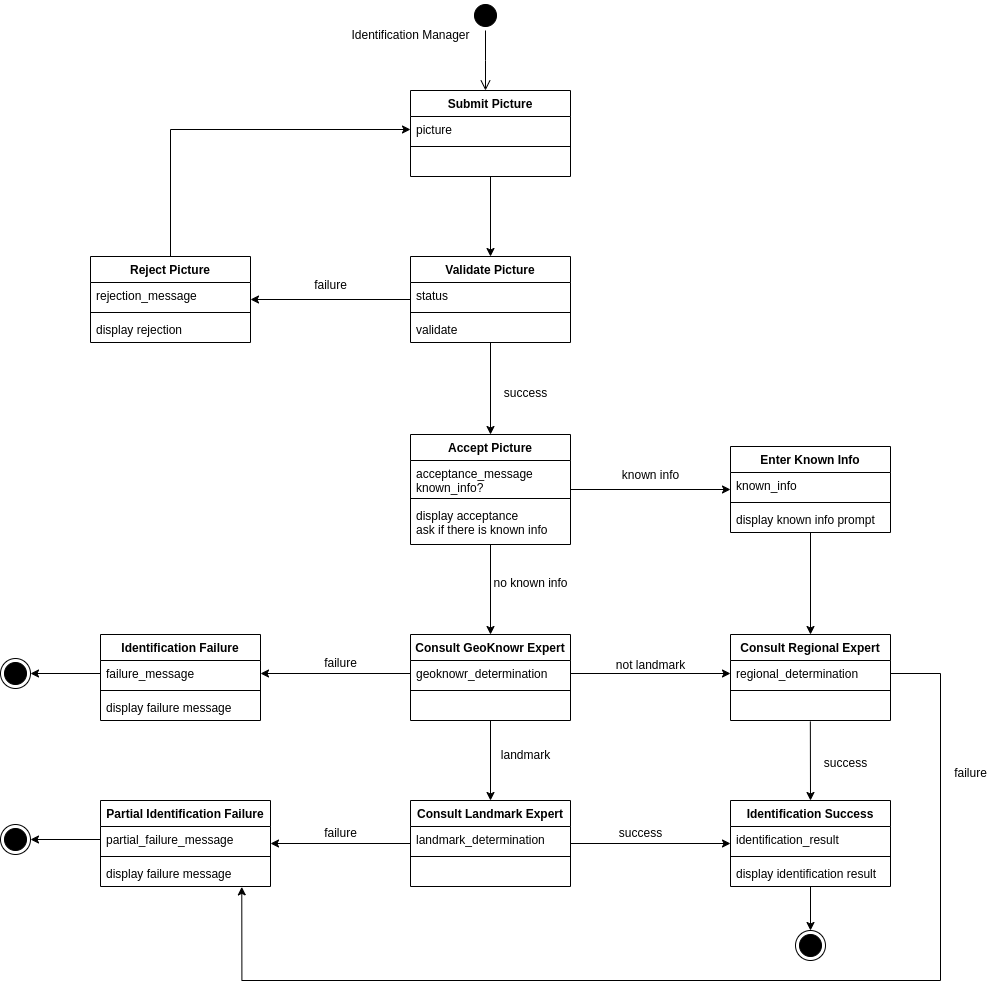
\includegraphics[width=1\linewidth]{ident_mng_state_diag.png}
    \textbf{\caption{Identification Manager State Diagram}}
    \label{fig:ident_mng}
\end{figure}

\begin{figure}[H]
    \centering
    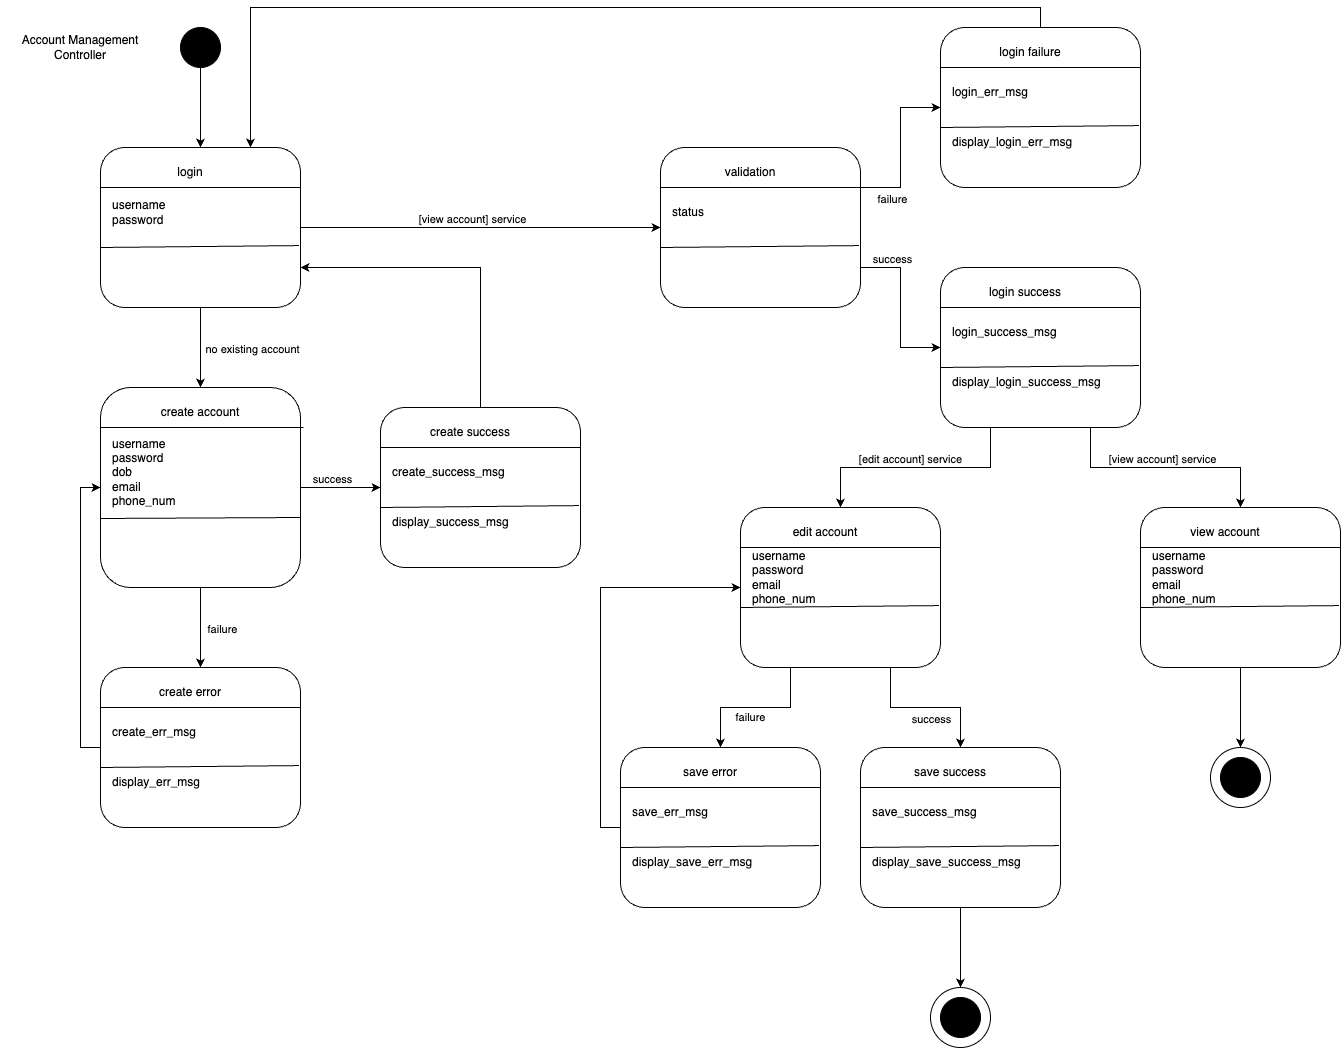
\includegraphics[width=1\linewidth]{AccountController.drawio.png}
    \textbf{\caption{Account Manager State Diagram}}
    \label{fig:acct_mng}
\end{figure}

\begin{figure}[H]
    \centering
    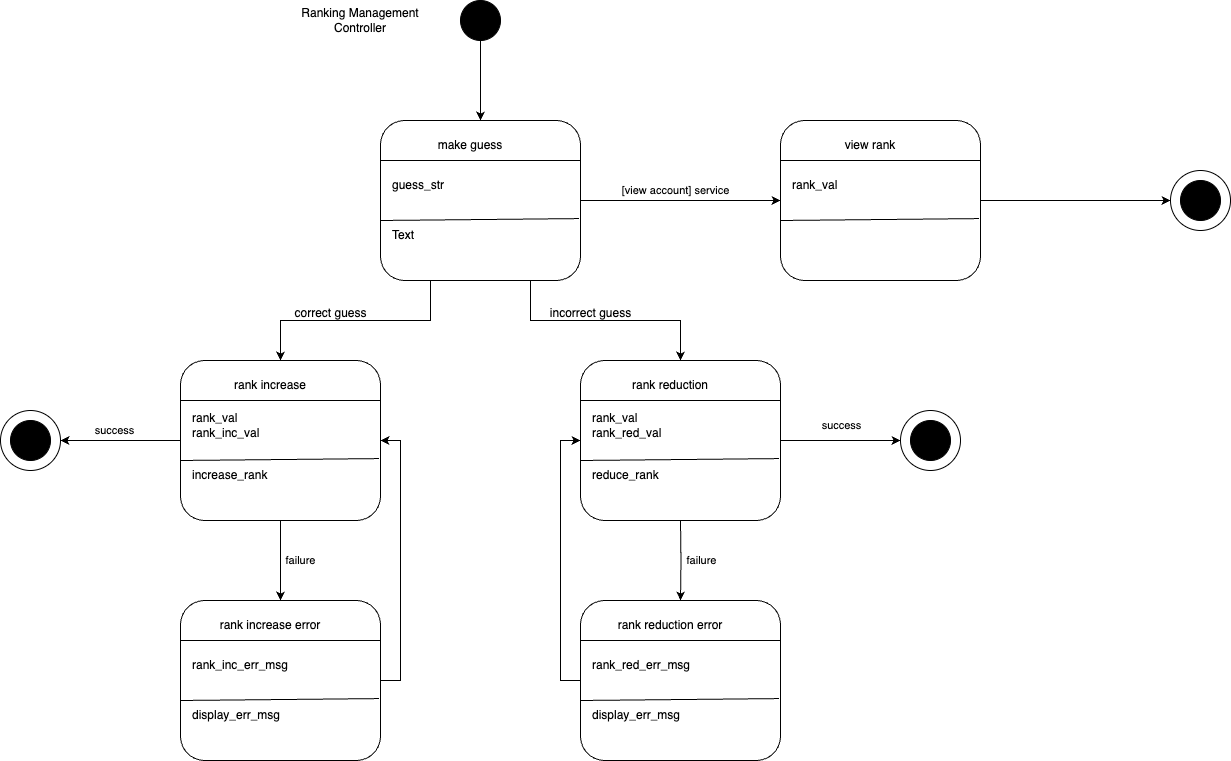
\includegraphics[width=1\linewidth]{RankingController.drawio.png}
    \textbf{\caption{Ranking Manager State Diagram}}
    \label{fig:rank_mng}
\end{figure}

% End Section

\section{Sequence Diagrams}
\label{sec:sequence_diagrams}
% Begin Section
This section should provide a sequence diagram for each use case of your application.

\text{5 diagrams total (see D1 Functional Requirements for use cases)}

\begin{figure}[H]
    \centering
    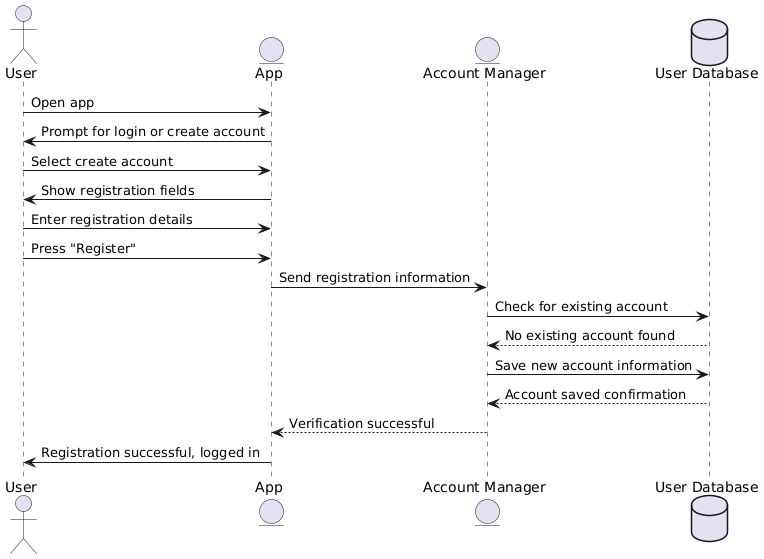
\includegraphics[width=0.6\textwidth]{out/sequence1/sequence1.png} % replace image with diagram
    \caption{Register Account Sequence Diagram}
\end{figure}

\begin{figure}[H]
    \centering
    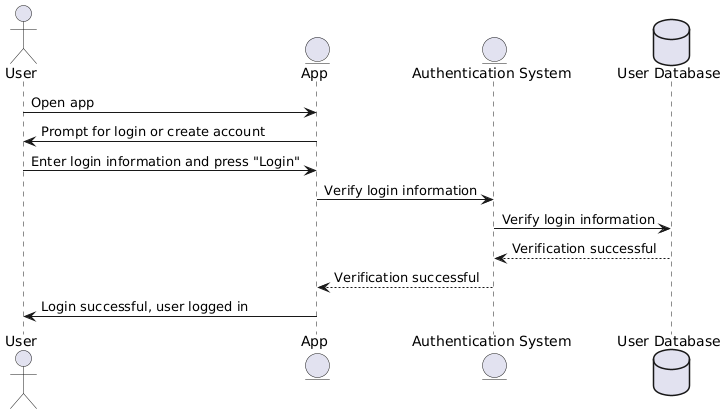
\includegraphics[width=0.6\textwidth]{out/sequence2/sequence2.png} % replace image with diagram
    \caption{Log in Sequence Diagram}
\end{figure}

% SPLIT HERE

\begin{figure}[H]
    \centering
    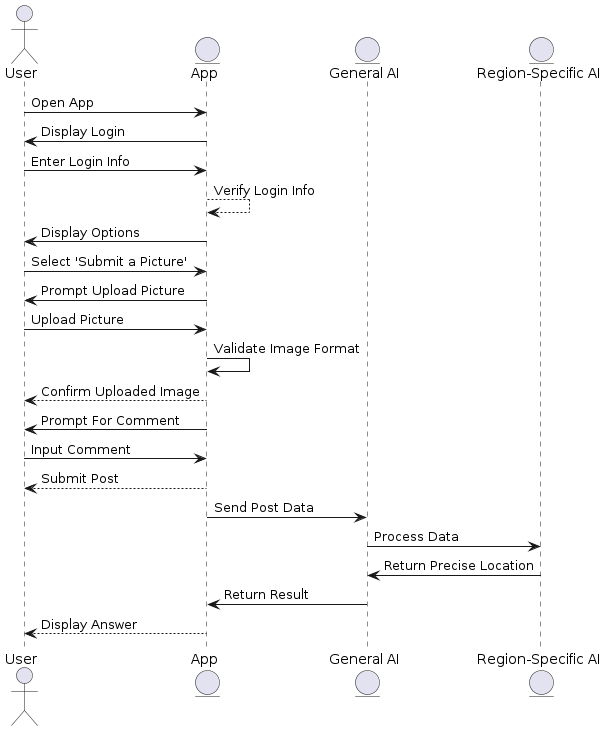
\includegraphics[width=0.6\textwidth]{out/sequence3/sequence3.png} % replace image with diagram
    \caption{Submit Picture (Non-Regional) Sequence Diagram}
\end{figure}

\begin{figure}[H]
    \centering
    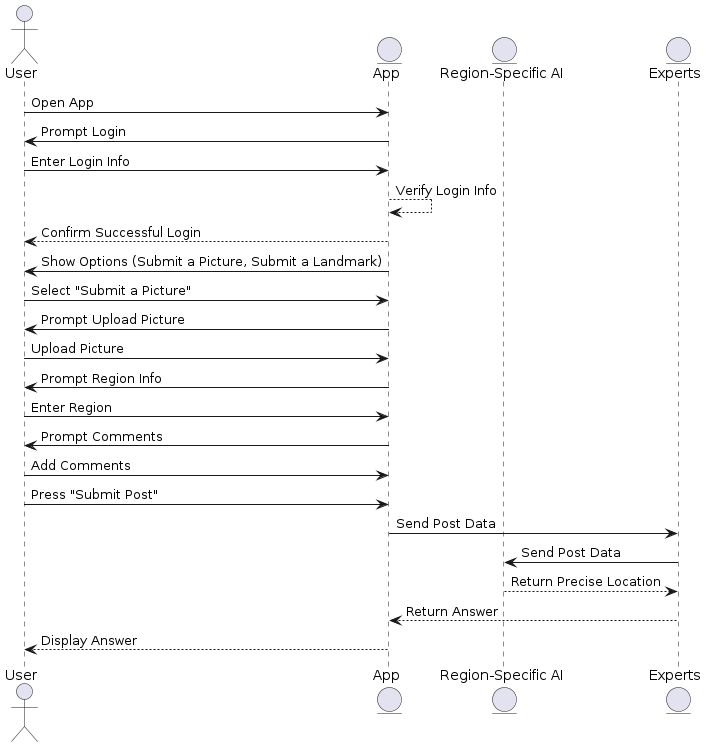
\includegraphics[width=0.7\textwidth]{out/sequence4/sequence4.png} % replace image with diagram
    \caption{Submit Picture (Regional) Sequence Diagram}
\end{figure}

\begin{figure}[H]
    \centering
    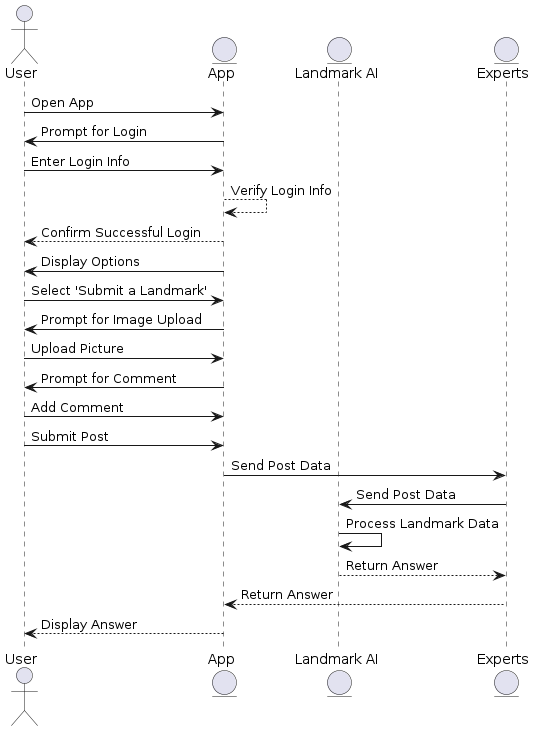
\includegraphics[width=0.5\textwidth]{out/sequence5/sequence5.png} % replace image with diagram
    \caption{Submit Picture (Landmark) Sequence Diagram}
\end{figure}


% End Section

\section{Detailed Class Diagram}
\label{sec:detailed_class_diagram}
% Begin Section
This section should provide a detailed class diagram for your application.
% End Section

\appendix
\section{Division of Labour}
\label{sec:division_of_labour}
% Begin Section
\textbf{Nesbitt, Matthew:}
\begin{itemize}
    \item
\end{itemize}

\includegraphics[scale=0.15]{mattsignature.jpg}

\textbf{Klisuric, Petar:}
\begin{itemize}
  \item   
\end{itemize}

\includegraphics[scale=0.15]{petarsignature.jpg}

\textbf{Rooprai, Mankaran:}
\begin{itemize}
    \item
\end{itemize}

\includegraphics[scale=0.15]{mankaransignature.png}

\textbf{Nielsen, Claire}
\begin{itemize}
    \item 2.2 Account Manager State Diagram
    \item 2.3 Ranking Manager State Diagram
\end{itemize}

\includegraphics[scale=0.15]{clairesignature.jpg}

\textbf{Bornomala, Anindita}
\begin{itemize}
    \item Created \textbf{Submit Picture (Non-Regional)} Sequence Diagram
    \item Created \textbf{Submit Picture (Regional)} Sequence Diagram
    \item Created \textbf{Submit Picture (Landmark)} Sequence Diagram
\end{itemize}

\includegraphics[scale=0.50]{bornosignature.png}

\textbf{Lam, Robert}
\begin{itemize}
    \item
\end{itemize}

\includegraphics[scale=1]{robertsignature.png}

% End Section

\newpage
\section*{IMPORTANT NOTES}
\begin{itemize}
	\item You do \underline{NOT} need to provide a text explanation of each diagram; the diagram should speak for itself
	\item Please document any non-standard notations that you may have used
	\begin{itemize}
		\item \emph{Rule of Thumb}: if you feel there is any doubt surrounding the meaning of your notations, document them
	\end{itemize}
	\item Some diagrams may be difficult to fit into one page
	\begin{itemize}
		\item It is OK if the text is small but please ensure that it is readable when printed
		\item If you need to break a diagram onto multiple pages, please adopt a system of doing so and throughly explain how it can be reconnected from one page to the next; if you are unsure about this, please ask me
	\end{itemize}
	\item Please submit the latest version of Deliverable 1 and Deliverable 2 with Deliverable 3
	\begin{itemize}
		\item They do not have to be a freshly printed versions; the latest marked versions are OK
	\end{itemize}
	\item If you do \underline{NOT} have a Division of Labour sheet, your deliverable will \underline{NOT} be marked
\end{itemize}


\end{document}
%------------------------------------------------------------------------------
